\documentclass[conference]{IEEEtran}

\usepackage[T1]{fontenc}
\usepackage{newtxtext,newtxmath}
\usepackage{graphicx}
\usepackage{booktabs}
\usepackage{array}
\newcolumntype{P}[1]{>{\raggedright\arraybackslash}p{#1}}
\usepackage{listings}
\usepackage{xcolor}
\usepackage{tikz}
\usetikzlibrary{arrows.meta,positioning,calc}
\usepackage{url}
\usepackage[hidelinks]{hyperref}

% No hyphenation anywhere: words are never split across lines.
\hyphenpenalty=10000
\exhyphenpenalty=10000
\tolerance=3000
\emergencystretch=3em
\sloppy

\definecolor{codebg}{RGB}{247,245,240}
\definecolor{codekw}{RGB}{176,30,100}
\definecolor{codecm}{RGB}{110,110,110}
\lstdefinestyle{turtle}{
  basicstyle=\ttfamily\scriptsize,
  backgroundcolor=\color{codebg},
  frame=single, rulecolor=\color{codebg},
  framesep=3pt, xleftmargin=3pt, xrightmargin=3pt,
  columns=fullflexible, keepspaces=true,
  breaklines=true, breakatwhitespace=true,
  keywordstyle=\color{codekw}\bfseries,
  commentstyle=\color{codecm}\itshape,
  morekeywords={SET,PEN,PENUP,PENDOWN,MOVE,TURN,REPEAT},
  morecomment=[l]{\#},
  literate={-}{{$-$}}1 {->}{{$\rightarrow$}}2 {<=}{{$\le$}}1,
  showstringspaces=false
}
\lstdefinestyle{plain}{
  basicstyle=\ttfamily\scriptsize,
  backgroundcolor=\color{codebg},
  frame=single, rulecolor=\color{codebg},
  framesep=3pt, xleftmargin=3pt, xrightmargin=3pt,
  columns=fullflexible, keepspaces=true,
  breaklines=true, breakatwhitespace=true,
  literate={-}{{$-$}}1 {->}{{$\rightarrow$}}2 {<=}{{$\le$}}1,
  escapeinside={(*}{*)},
  showstringspaces=false
}

\newcommand{\code}[1]{\texttt{#1}}

\begin{document}

\title{Turtle Compiler: An Interactive Six Phase Compiler\\for a Turtle Graphics Language}

\author{\IEEEauthorblockN{C Murali Madhav, Pugazhendhi J, Tejmul Movin, J Amathziah, Ravi Yadav}
\IEEEauthorblockA{Newton School of Technology, Rishihood University, India}}

\maketitle

{\small\bfseries\noindent\textit{Abstract:} Compiler courses teach six phases: lexical analysis, syntax analysis, semantic analysis, intermediate code generation, code optimization and code generation. Students usually meet each phase on its own small example, and rarely watch one program travel through all of them. We present Turtle Compiler, a complete compiler for a small turtle graphics language whose every phase is visible. The language has seven statements and a twelve rule LL(1) grammar. The compiler is a single JavaScript module of 659 lines with no dependencies. It tokenizes with ordered regular expressions, parses with a table driven LL(1) parser whose FIRST sets, FOLLOW sets and parse table are computed from the grammar, enforces eight semantic rules with a symbol table, emits three address code, applies six optimizations until a fixed point, and generates four byte machine code for a register based virtual machine that draws the picture. A website recompiles the program on every keystroke and shows the output of each phase; a command line tool, turtlec, runs the same module in a terminal. Every optimized program is run on the virtual machine against the unoptimized one, and the two drawings are compared line by line. On our example programs the optimizer removes up to 58\% of the instructions and 46\% of the machine steps with identical drawings, and a full compilation takes under 50 microseconds.\par}

\vspace{0.6em}
{\small\bfseries\noindent\textit{Index Terms:} compiler design, lexical analysis, LL(1) parsing, semantic analysis, three address code, code optimization, code generation, virtual machine, turtle graphics, computing education.\par}

\section{Introduction}

A compiler translates a program written by a person into instructions that a machine can run. Textbooks describe this translation as a pipeline of six phases \cite{aho2006,cooper2011}. Each phase is usually taught with its own small example: a regular expression for a lexer, an expression grammar for a parser, a basic block for an optimizer. What a student rarely sees is a single program entering at one end and leaving at the other, with the output of every phase in between.

We built Turtle Compiler to close that gap. Its source language is a turtle graphics language in the tradition of Logo \cite{papert1980,abelson1981}: a turtle holding a pen walks, turns and draws. We chose this domain for two reasons. First, the language can be very small, so the complete output of every phase fits on one screen. Second, the result is a picture, so anyone can tell at a glance whether the compiler worked.

This paper makes the following contributions.
\begin{itemize}
\item A small language with seven statements and an LL(1) grammar of twelve rules, with eight semantic rules and two warnings.
\item A compiler that implements all six phases in one dependency free JavaScript module, from regular expression scanning to machine code for a virtual machine.
\item An optimizer of six classic transformations whose correctness is checked on every compilation by running both versions of the program and comparing the drawings.
\item A website that recompiles on every keystroke and presents each phase with its rules and its output, and a command line compiler that shares the same module.
\item An evaluation on seven example programs, four valid and three that fail in a chosen phase.
\end{itemize}

The live website is available at \url{https://turtle.muralimadhav.com} and the source code at \url{https://github.com/HackHeroic/turtle-compiler}.

\section{Background and Related Work}

Turtle graphics began with Logo, designed to let children learn mathematics by programming a turtle \cite{papert1980}; Abelson and diSessa later developed turtle geometry as a medium for mathematics \cite{abelson1981}. Our language keeps the turtle and drops everything Logo has beyond drawing, because our goal is to teach compilation rather than programming.

The phases we implement follow the standard texts \cite{aho2006,cooper2011,muchnick1997}. Our parser is a predictive LL(1) parser; the alternative family, LR parsing, was introduced by Knuth \cite{knuth1965} and accepts more grammars at the cost of much larger tables. Our optimizer combines peephole optimization, introduced by McKeeman \cite{mckeeman1965}, with transformations over basic blocks in the sense of Allen \cite{allen1970}.

Interactive tools already support formal languages courses. JFLAP \cite{rodger2006}, for example, lets students build and simulate automata and grammars. Such tools focus on one formalism at a time. Our system instead shows how the formalisms connect: the regular expressions of phase one produce the tokens that the grammar of phase two consumes, and so on to machine code.

\section{The Turtle Language}

Table~\ref{tab:lang} lists the seven statements. A program is a sequence of statements; \code{REPEAT} blocks may nest. Lines that start with \code{\#} are comments. The pen starts down and white, at the origin, facing up.

\begin{table}[t]
\caption{Statements of the Turtle language}
\label{tab:lang}
\centering
\footnotesize
\begin{tabular}{@{}>{\ttfamily}l P{4.6cm}@{}}
\toprule
\textrm{\textbf{Statement}} & \textbf{Meaning and limits} \\
\midrule
MOVE n; & Move forward $n$ steps, drawing if the pen is down; $1 \le n \le 500$ \\
TURN n; & Turn right $n$ degrees, left if $n<0$; $-360 \le n \le 360$ \\
PEN c; & Choose one of 9 colours: RED, ORANGE, YELLOW, GREEN, CYAN, BLUE, PURPLE, PINK, WHITE \\
PENUP; & Lift the pen: move without drawing \\
PENDOWN; & Put the pen down again \\
SET x = n; & Name a constant; each name is set once \\
REPEAT n \{ \dots\ \} & Run the body $n$ times; $1 \le n \le 100$, nested at most 3 deep \\
\bottomrule
\end{tabular}
\end{table}

Listing~\ref{lst:star} shows the program we use as a running example. It draws a five pointed star. Two of its lines are wasteful on purpose, so that the optimizer has work to do: the first \code{PEN} is replaced before anything is drawn, and the two turns could be one.

\begin{lstlisting}[style=turtle, caption={The Star, our running example}, label={lst:star}, float=t]
# A pink star. Two lines here are wasteful on purpose:
# phase 5 cleans them up.
SET side = 150;
PEN BLUE;
PEN PINK;
REPEAT 5 {
  MOVE side;
  TURN 100;
  TURN 44;
}
\end{lstlisting}

\section{System Architecture}

Fig.~\ref{fig:pipeline} shows the pipeline. Each phase is a pure function in one module, \code{compiler/compiler.js}: \code{lex}, \code{parse}, \code{check}, \code{genIR}, \code{optimize}, \code{codegen} and the virtual machine \code{run}. A driver, \code{compile}, calls them in order and stops after the first phase that reports an error, because later phases would only work on a broken program. The same module is loaded by the website, which runs it in the browser, and by the command line tool, which runs it in Node.js. A rule fixed in the module is therefore fixed everywhere.

\begin{figure*}[t]
\centering
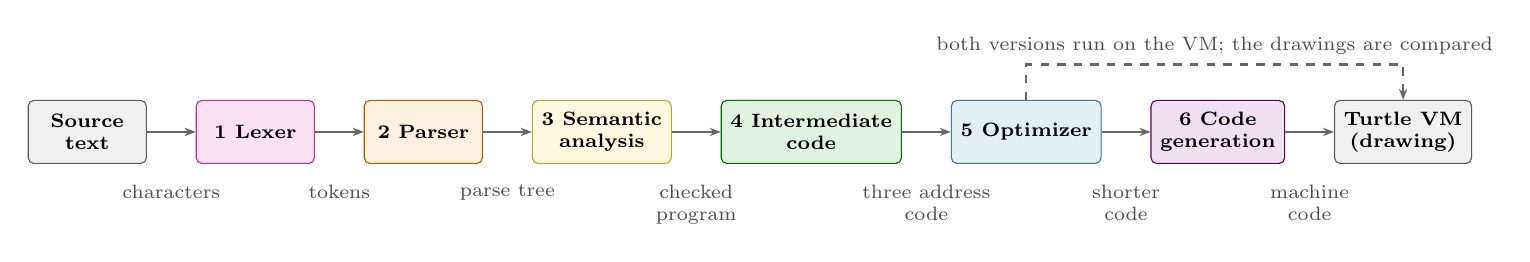
\begin{tikzpicture}[
  node distance=0.62cm,
  box/.style={draw, rounded corners=2pt, minimum height=0.8cm, minimum width=1.5cm, align=center, font=\scriptsize\bfseries, fill=#1!12, draw=#1!70!black},
  data/.style={font=\scriptsize, align=center, text=black!70},
  arr/.style={-{Stealth[length=4pt]}, thick, black!60}]
\node[box=gray] (src) {Source\\text};
\node[box=magenta, right=of src] (lex) {1 Lexer};
\node[box=orange, right=of lex] (par) {2 Parser};
\node[box=yellow!70!orange, right=of par] (sem) {3 Semantic\\analysis};
\node[box=green!60!black, right=of sem] (ir) {4 Intermediate\\code};
\node[box=cyan!70!black, right=of ir] (opt) {5 Optimizer};
\node[box=violet, right=of opt] (gen) {6 Code\\generation};
\node[box=gray, right=of gen] (vm) {Turtle VM\\(drawing)};
\foreach \a/\b/\t in {src/lex/characters, lex/par/tokens, par/sem/parse tree, sem/ir/checked\\program, ir/opt/three address\\code, opt/gen/shorter\\code, gen/vm/machine\\code} {
  \draw[arr] (\a) -- (\b);
  \node[data, below=4pt] at ($(\a.south east)!0.5!(\b.south west)$) {\t};
}
\draw[arr, dashed] (opt.north) -- ++(0,0.45) -| node[data, pos=0.25, above] {both versions run on the VM; the drawings are compared} (vm.north);
\end{tikzpicture}
\caption{The six phases. Each arrow carries the output of one phase into the next. The optimizer's result is checked by running the original and the optimized code on the virtual machine and comparing the two drawings.}
\label{fig:pipeline}
\end{figure*}

\begin{figure*}[t]
\centering
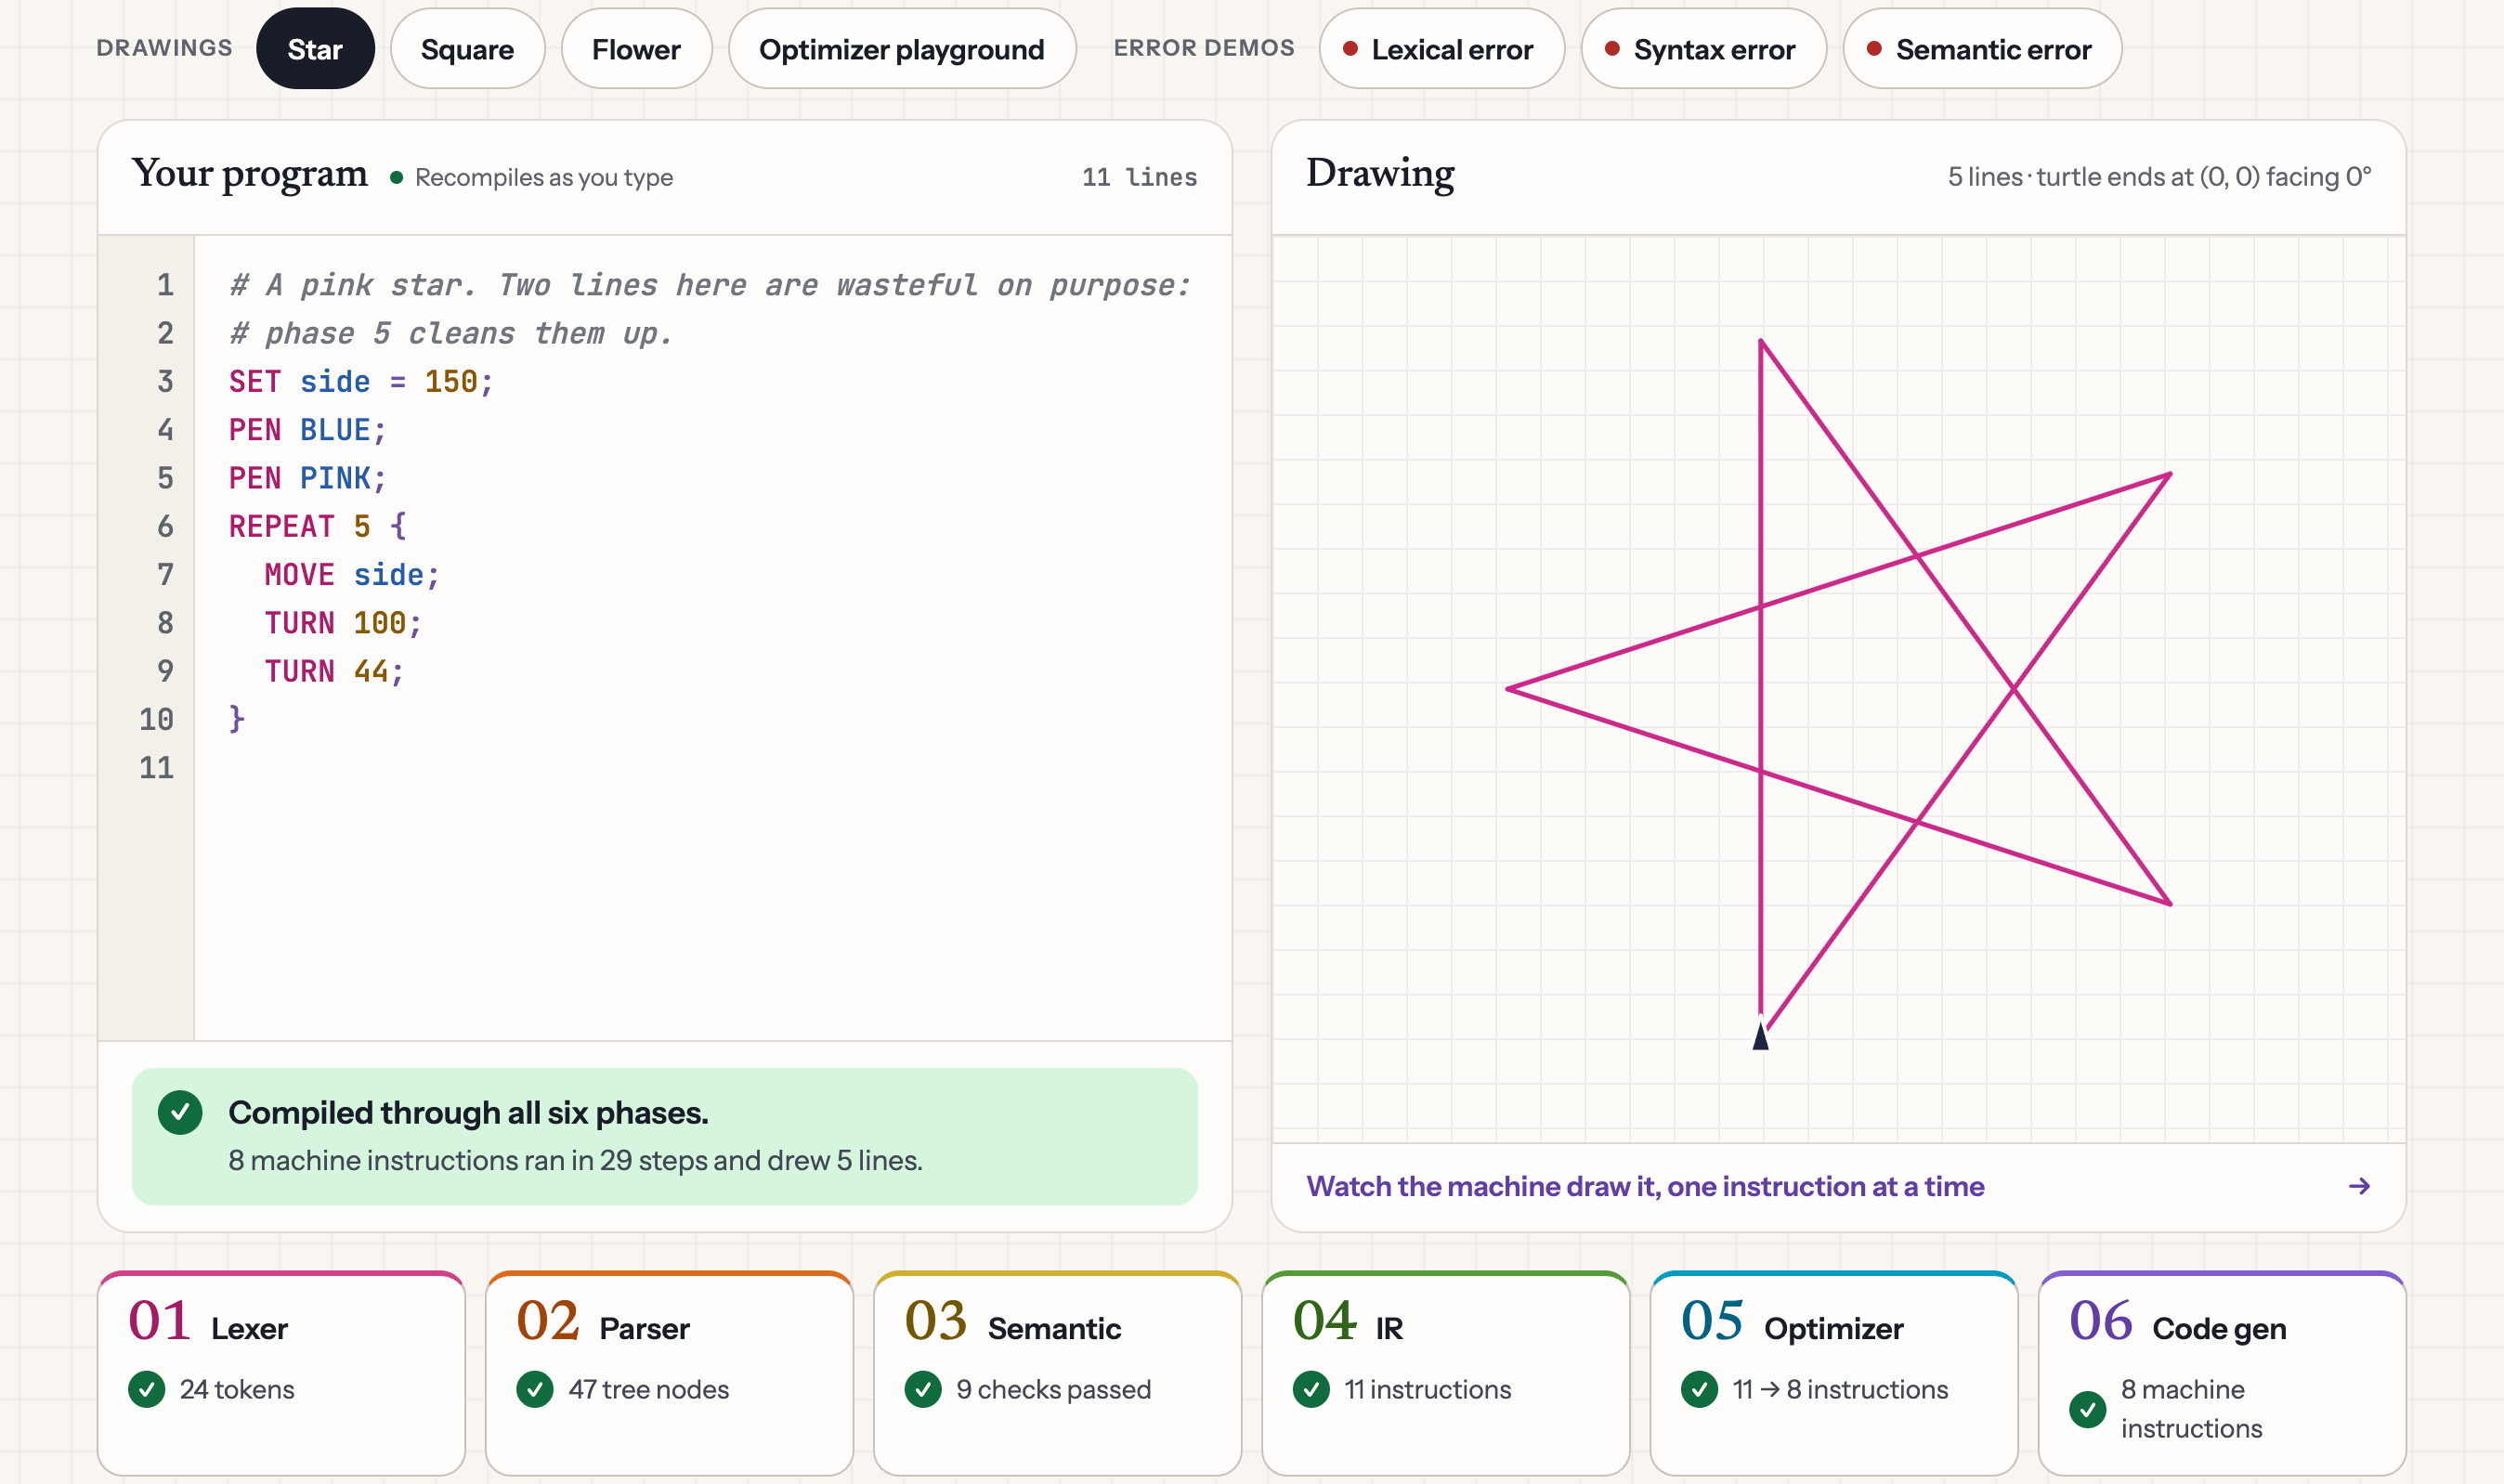
\includegraphics[width=\textwidth]{figures/workbench.png}
\caption{The workbench on the website, compiling the Star. Each keystroke reruns all six phases. The status panel summarizes the run (8 machine instructions, 29 steps, 5 lines), and the six cards below report what each phase produced.}
\label{fig:workbench}
\end{figure*}

The website (Fig.~\ref{fig:workbench}) has an editor, the drawing, a status panel, and one card per phase. Each card has two halves: the rules the phase applies, and what the phase made from the current program. Buttons load the example programs, including three error demonstrations, one for each phase that can reject a program.

\section{The Six Phases}

\subsection{Lexical Analysis}

The lexer turns characters into tokens. It holds an ordered list of regular expressions: whitespace, comments, numbers (\code{$-$?[0-9]+}), words, and the four symbols \code{\{}, \code{\}}, \code{;} and \code{=}. At each position it tries the rules in order and takes the first that matches; because each expression is greedy, the match is the longest possible, so \code{150} is one number and \code{PENDOWN} is one word rather than \code{PEN} followed by \code{DOWN}. A word becomes a keyword if it is one of the seven commands, compared without regard to case, and an identifier otherwise. Whitespace and comments are skipped.

Every token keeps its line and column, so that any later phase can point at the exact place of an error. An unknown character is reported and skipped, and scanning continues, so all lexical errors are reported together. A minus sign followed by a space gets a dedicated message, \emph{a minus sign must touch its number}, because \code{TURN $-$ 90} is the most common slip. At the end the lexer appends an end marker, \code{\$}, which the parser needs. The Star yields 25 tokens, the end marker included (Fig.~\ref{fig:lexer}).

\begin{figure}[t]
\centering
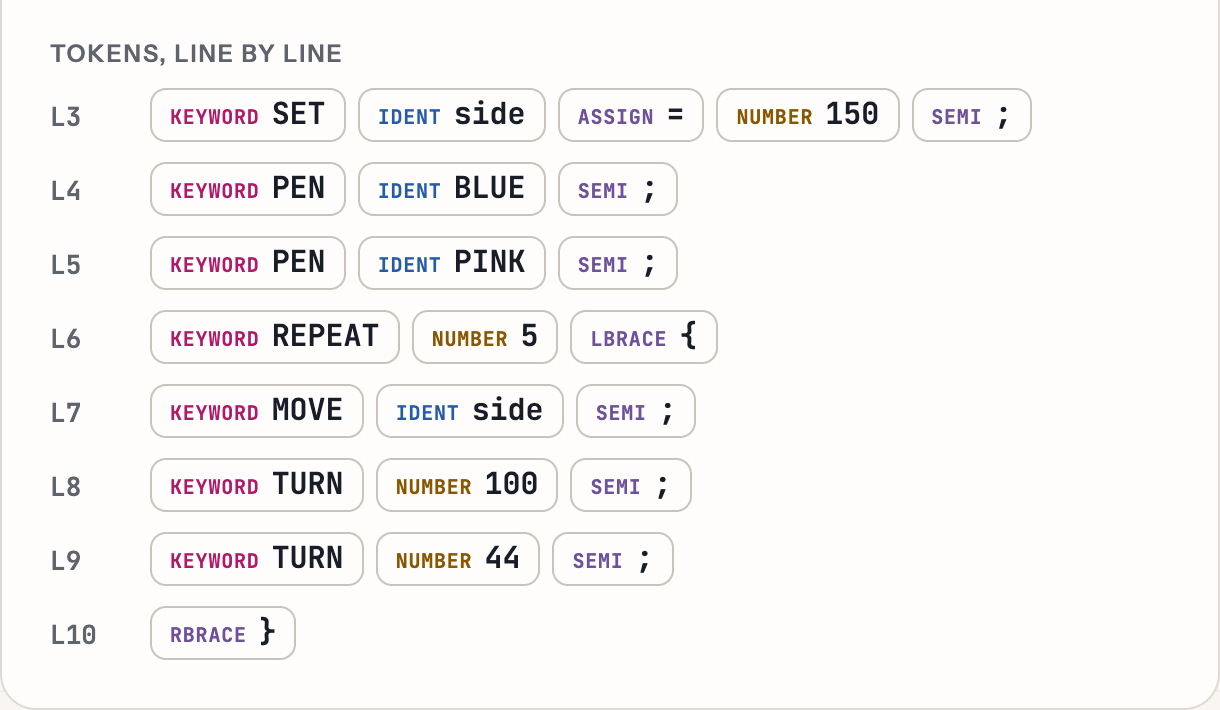
\includegraphics[width=\columnwidth]{figures/lexer-tokens.png}
\caption{Tokens of the Star, line by line, as the lexer card shows them. Each chip gives the token type and its text.}
\label{fig:lexer}
\end{figure}

\subsection{Syntax Analysis}

Listing~\ref{lst:grammar} gives the grammar. Two design choices make it LL(1). Every statement begins with its own keyword, so one token of lookahead always selects the rule. The statement list is right recursive rather than left recursive, since a top down parser would loop forever on a left recursive rule; the empty rule~3 lets a list end, both at the end of the program and at the brace that closes a loop.

\begin{lstlisting}[style=plain, caption={The grammar: twelve rules}, label={lst:grammar}, float=t]
 1 program   -> stmt_list
 2 stmt_list -> stmt stmt_list
 3 stmt_list -> (*$\varepsilon$*)
 4 stmt      -> MOVE value ;
 5 stmt      -> TURN value ;
 6 stmt      -> PEN IDENT ;
 7 stmt      -> PENUP ;
 8 stmt      -> PENDOWN ;
 9 stmt      -> SET IDENT = NUMBER ;
10 stmt      -> REPEAT value { stmt_list }
11 value     -> NUMBER
12 value     -> IDENT
\end{lstlisting}

The parser does not contain a hand written table. At load time the module computes FIRST and FOLLOW for every nonterminal by iterating until no set changes, then fills the parse table $M[A,a]$ with the standard construction \cite{aho2006}: rule $p$ for $A$ goes in every column of FIRST of its right side, and also in every column of FOLLOW($A$) when its right side can derive the empty string. Any cell that receives two rules is recorded as a conflict. For this grammar there are none; Table~\ref{tab:ll1} shows the result.

\begin{table*}[t]
\caption{The LL(1) parse table $M[A,a]$ computed from the grammar. A cell holds the number of the rule to apply when $A$ is on top of the stack and $a$ is the next token. Empty cells are syntax errors; the columns for \texttt{\{}, \texttt{;} and \texttt{=} are empty in every row and are omitted.}
\label{tab:ll1}
\centering
\footnotesize
\begin{tabular}{@{}l *{11}{c}@{}}
\toprule
$A$ \textbackslash\ $a$ & \texttt{MOVE} & \texttt{TURN} & \texttt{PEN} & \texttt{PENUP} & \texttt{PENDOWN} & \texttt{SET} & \texttt{REPEAT} & \texttt{NUMBER} & \texttt{IDENT} & \texttt{\}} & \texttt{\$} \\
\midrule
\texttt{program}   & 1 & 1 & 1 & 1 & 1 & 1 & 1 &    &    &   & 1 \\
\texttt{stmt\_list} & 2 & 2 & 2 & 2 & 2 & 2 & 2 &    &    & 3 & 3 \\
\texttt{stmt}      & 4 & 5 & 6 & 7 & 8 & 9 & 10 &   &    &   &   \\
\texttt{value}     &   &   &   &   &   &   &    & 11 & 12 &   &   \\
\bottomrule
\end{tabular}
\end{table*}

Parsing uses an explicit stack that starts as \code{\$ program}. At each step the parser compares the top of the stack with the next token. If the top is a terminal equal to the token, both are consumed (\emph{match}). If the top is a nonterminal, it is replaced by the right side of the rule found in the table, pushed in reverse so that its first symbol is on top (\emph{expand}). An empty cell or a failed match is a syntax error, reported with what was expected and what was found, for example \emph{Expected ; after "100" but found "TURN"}. Words that beginners bring from other languages, such as \code{FORWARD} or \code{LOOP}, receive a suggestion. The parser stops at the first syntax error. The Star is accepted in 46 steps and yields a parse tree of 47 nodes; every step is recorded, and the website shows the trace (Fig.~\ref{fig:trace}). The parse tree is then reduced to an abstract syntax tree with one node per statement.

\begin{figure}[t]
\centering
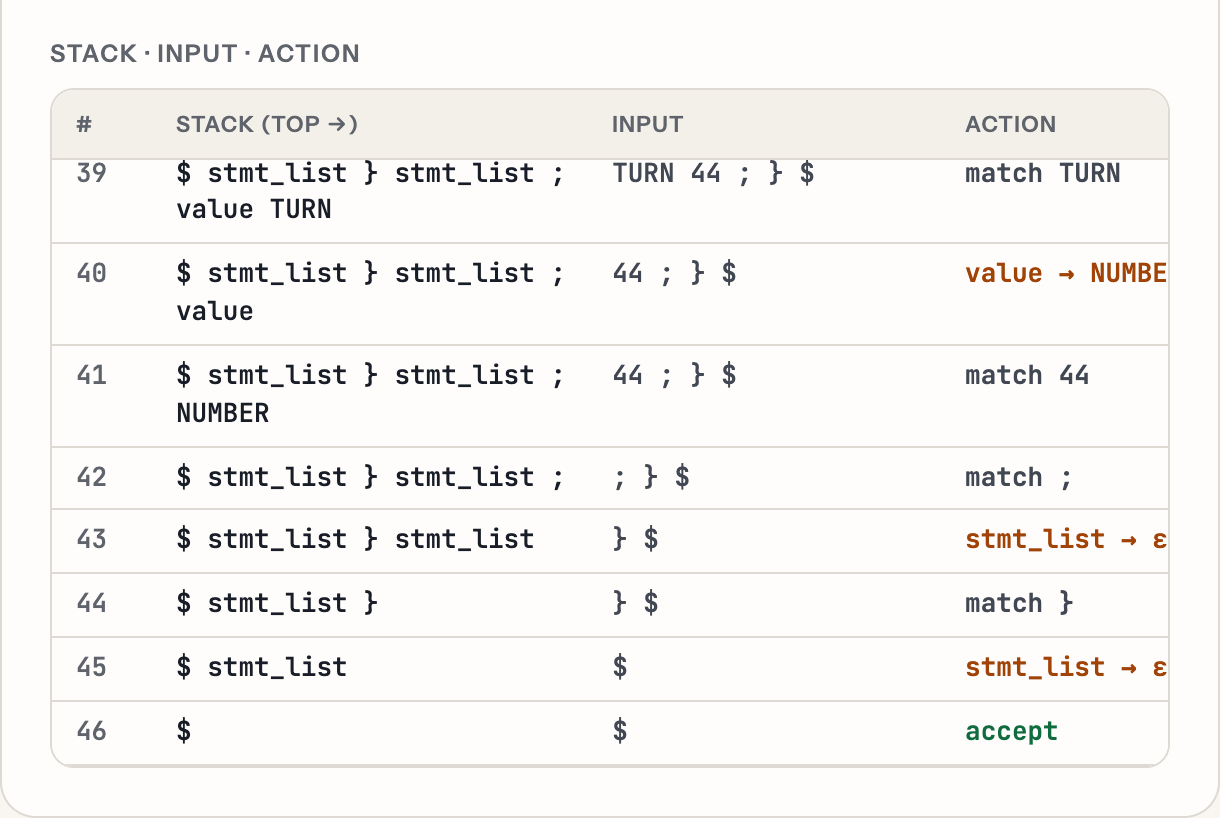
\includegraphics[width=\columnwidth]{figures/parser-trace.png}
\caption{The last steps of the parse of the Star. The stack grows to the right. Each row either expands the nonterminal on top using the table or matches a token; the final row accepts.}
\label{fig:trace}
\end{figure}

\subsection{Semantic Analysis}

A grammar describes the shape of a program but cannot remember earlier lines or compare numbers. \code{PEN GOLD;} fits rule~6, yet \code{GOLD} is not a colour. The semantic phase walks the abstract syntax tree in program order, records every \code{SET} in a symbol table, and applies the rules in Table~\ref{tab:sem}. Errors stop the compiler before phase four; warnings do not. All semantic errors are reported together, since each check stands alone (Fig.~\ref{fig:sem}). The Star passes nine checks, and its symbol table holds one entry: \code{side}, value 150, set on line 3 and used on line 7.

\begin{table}[t]
\caption{Semantic rules and the reason for each}
\label{tab:sem}
\centering
\footnotesize
\begin{tabular}{@{}l P{2.5cm} P{3.7cm}@{}}
\toprule
\textbf{Rule} & \textbf{Check} & \textbf{Reason} \\
\midrule
S1 & A name is set before use & A name without a value cannot be drawn; catches typing mistakes \\
S2 & A name is set once & Names are constants; the optimizer relies on a single value \\
S3 & \code{PEN} takes one of 9 colours & The machine knows only these colours \\
S4 & \code{MOVE} in 1 to 500 & Zero draws nothing; 500 keeps the drawing on the canvas \\
S5 & \code{TURN} in $-360$ to 360 & More than a full turn is pointless \\
S6 & \code{REPEAT} in 1 to 100 & Zero is a mistake; the cap keeps runs short \\
S7 & Nesting at most 3 deep & The machine has three loop registers \\
S8 & A colour is not a variable name & \code{PEN RED} would be ambiguous \\
W1 & A set name is never used & Harmless but probably unintended \\
W2 & A loop has an empty body & Harmless; the optimizer removes it \\
\bottomrule
\end{tabular}
\end{table}

\begin{figure}[t]
\centering
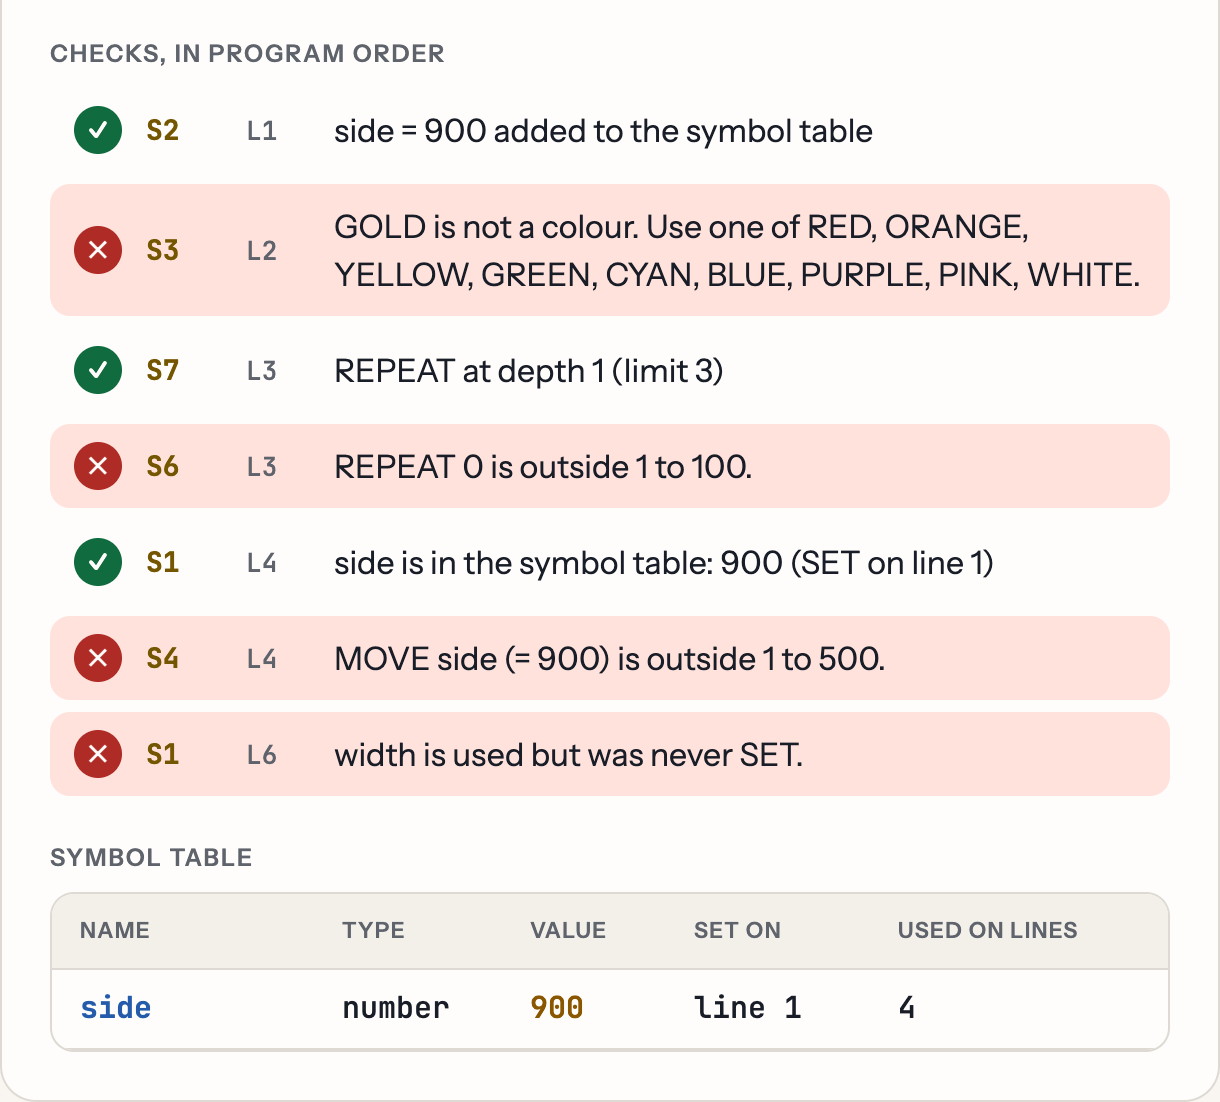
\includegraphics[width=\columnwidth]{figures/semantic-error.png}
\caption{The semantic error demonstration. Checks appear in program order; four rules fail (S3, S6, S4, S1) and all four are reported in one run. The symbol table is shown below the checks.}
\label{fig:sem}
\end{figure}

\subsection{Intermediate Code Generation}

The checked program is translated into three address code: instructions with at most two operands and one result. Simple statements map one to one: \code{SET} becomes a copy, \code{MOVE} becomes \code{move}, \code{PEN} becomes \code{color}. A loop has no single instruction, so each \code{REPEAT} is expanded by the template in Listing~\ref{lst:repeat}, with a fresh temporary as its counter and two fresh labels. Fresh names skip any name the program sets, so a user constant called \code{t1} cannot clash with a temporary. A \code{halt} closes the program. Names are kept as names at this stage; replacing them with values is left to the optimizer, so that each phase does one job.

\begin{lstlisting}[style=plain, caption={Template for \texttt{REPEAT v \{ S \}}}, label={lst:repeat}, float=t]
      t = v                  counter starts
Ltop:                        top of the loop
      if t <= 0 goto Lout    leave when done
      ... S ...              the body
      t = t - 1              count down
      goto Ltop              go round again
Lout:                        after the loop
\end{lstlisting}

The Star becomes 13 lines: 11 instructions and 2 labels (Fig.~\ref{fig:ir}). The same code is also produced as quadruples (operator, two arguments, result) and divided into basic blocks, whose leaders are the first instruction, every label, and every instruction after a jump \cite{allen1970}. The Star has four blocks: setup, loop test, loop body, and exit.

\begin{figure}[t]
\centering
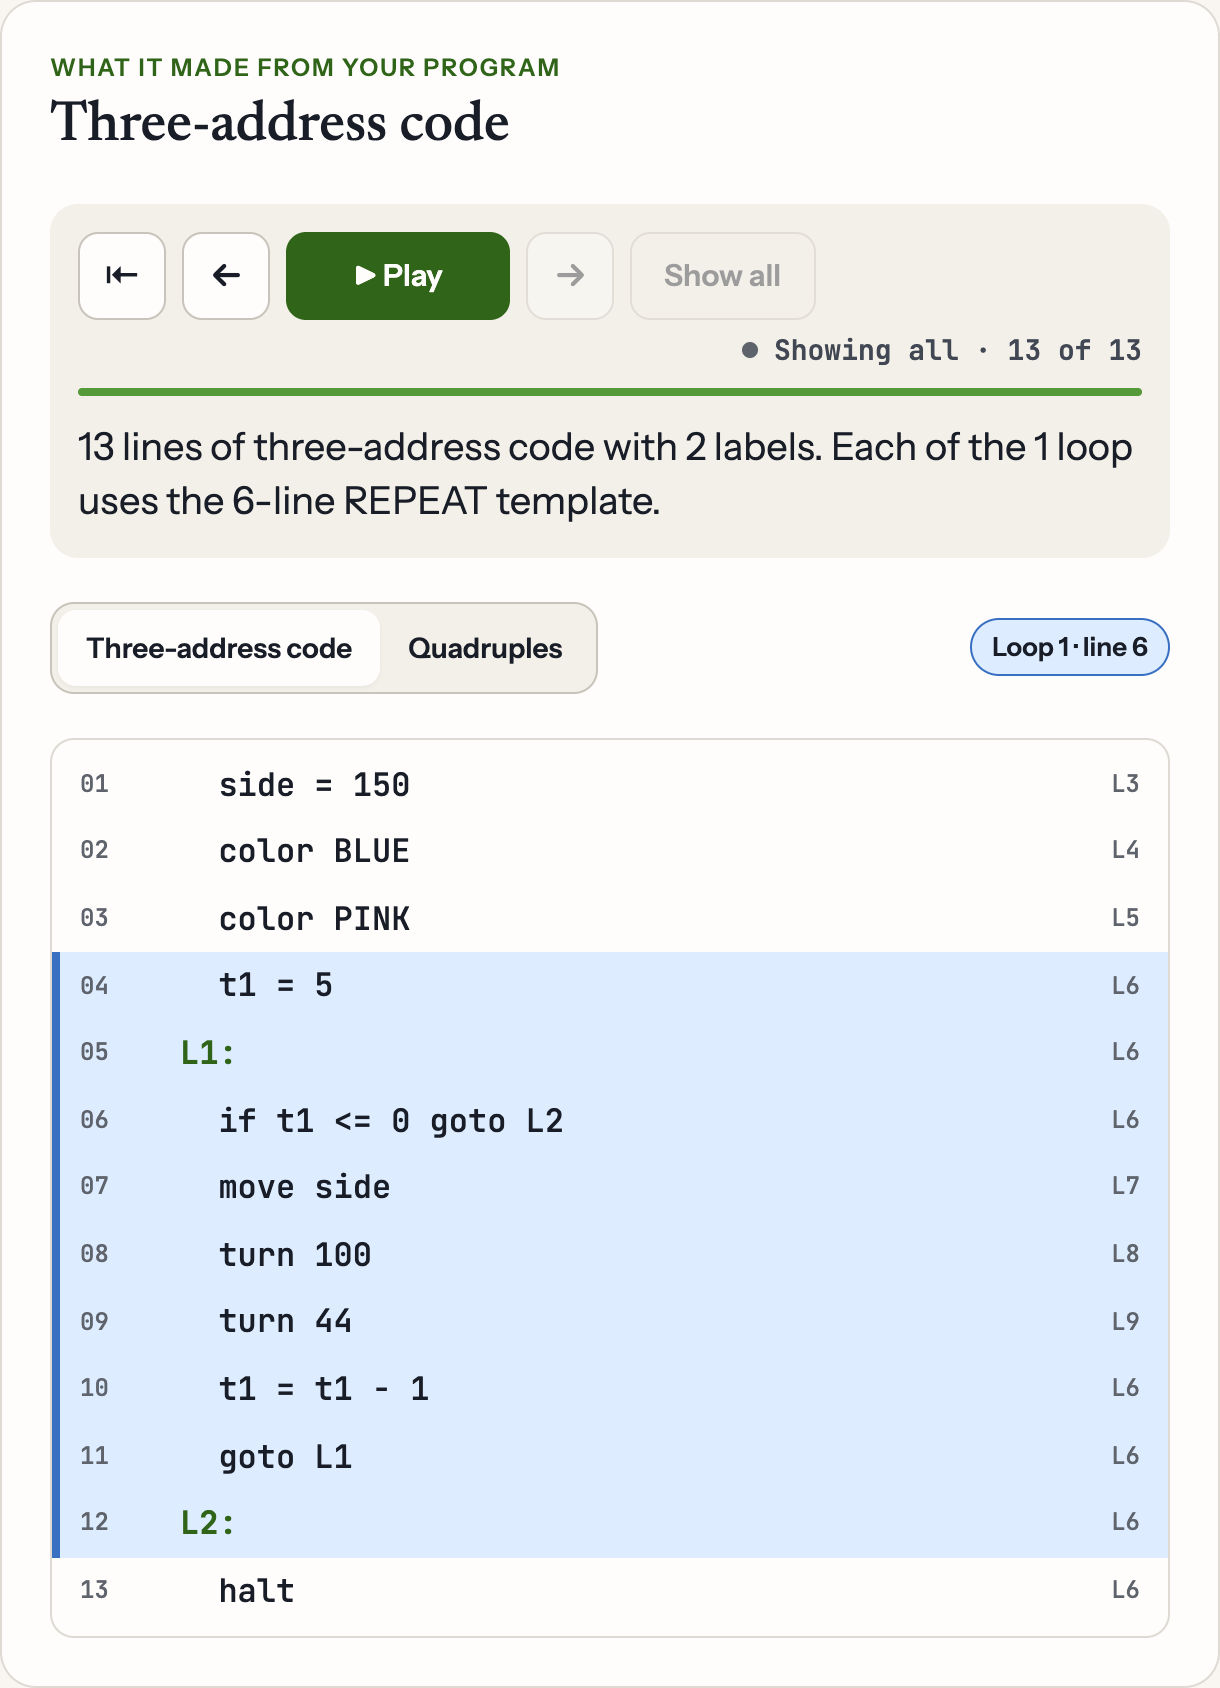
\includegraphics[width=\columnwidth, trim={0 0 0 720}, clip]{figures/ir.png}
\caption{Three address code for the Star. The shaded rows are the loop built from the template; the right column gives the source line of each instruction.}
\label{fig:ir}
\end{figure}

\subsection{Code Optimization}

The optimizer applies the six rules of Table~\ref{tab:opt} repeatedly until a full pass changes nothing, with a limit of 60 passes. Repetition matters because one change enables another: once constant propagation has replaced every use of \code{side} with 150, the copy \code{side = 150} has no readers, and dead code elimination removes it on the next pass. After every change the optimizer stores a snapshot, which lets the website step through the changes one at a time.

\begin{table}[t]
\caption{Optimization rules}
\label{tab:opt}
\centering
\footnotesize
\begin{tabular}{@{}l P{2.3cm} P{3.9cm}@{}}
\toprule
\textbf{Rule} & \textbf{Name} & \textbf{Effect} \\
\midrule
O1 & Constant propagation & Replace a set name with its value: \code{move side} becomes \code{move 150} \\
O2 & Dead code elimination & Delete a copy nobody reads, or a colour or pen change replaced before anything is drawn \\
O3 & Redundant code removal & Delete a change to the current state, or a full turn \\
O4 & Peephole merge \cite{mckeeman1965} & Join neighbouring moves or turns; rewrite a turn above 180 degrees as the shorter equivalent \\
O5 & Loop simplification & Delete an empty loop; replace a loop that runs once by its body \\
O6 & Code motion & Move a pen setting that is set once at the top of a loop body to just before the loop \\
\bottomrule
\end{tabular}
\end{table}

Correctness is not assumed. After optimizing, the compiler generates machine code for both the original and the optimized program and runs both on the virtual machine. It then normalizes each drawing, dropping segments of zero length and joining consecutive segments of the same colour that continue in the same direction, since merging two moves turns two segments into one. Finally it compares the two lists segment by segment, colour and both end points, within a tolerance of one part in a million. The result is shown on every compilation (Fig.~\ref{fig:opt}). On the Star the optimizer makes four changes in two passes: O1 replaces \code{side}, O2 deletes the unused copy and the overridden \code{color BLUE}, and O4 merges \code{turn 100} and \code{turn 44} into \code{turn 144}.

\begin{figure}[t]
\centering
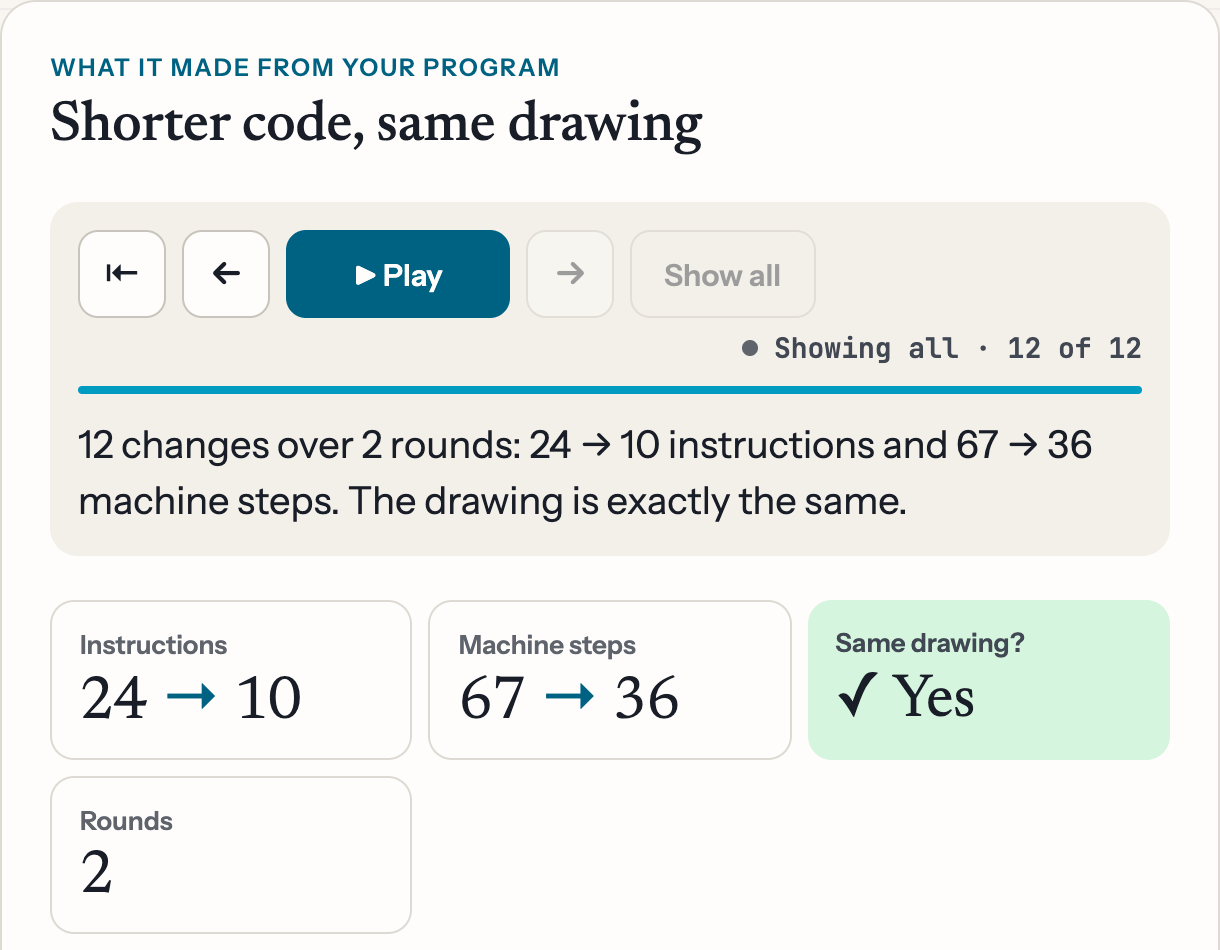
\includegraphics[width=\columnwidth]{figures/optimizer-top.png}
\caption{The optimizer card on the optimizer playground program: 12 changes over 2 passes reduce 24 instructions to 10 and 67 machine steps to 36, with an identical drawing.}
\label{fig:opt}
\end{figure}

\subsection{Code Generation and the Turtle VM}

The final phase targets the Turtle VM, a register machine with a program counter, three registers R1 to R3, and the turtle state: position, heading, pen and colour. Its instruction set has eleven instructions (Table~\ref{tab:isa}). Every instruction occupies four bytes: the opcode, a register number, and a sixteen bit operand in two bytes. A fixed size makes addressing trivial, and sixteen bits hold the largest operand, 500. \code{FWD \#150}, for example, is encoded as \code{10 00 00 96}.

\begin{table}[t]
\caption{Instruction set of the Turtle VM}
\label{tab:isa}
\centering
\footnotesize
\begin{tabular}{@{}c l P{4.4cm}@{}}
\toprule
\textbf{Opcode} & \textbf{Form} & \textbf{Effect} \\
\midrule
10 & \code{FWD n} & Move forward $n$, drawing if the pen is down \\
11 & \code{RGT n} & Turn right $n$ degrees \\
12 & \code{LFT n} & Turn left $n$ degrees \\
20 & \code{COL c} & Set the colour to colour number $c$ \\
21 & \code{PUP} & Pen up \\
22 & \code{PDN} & Pen down \\
30 & \code{LDI R, n} & Load $n$ into register R \\
31 & \code{DEC R} & Subtract 1 from register R \\
40 & \code{JLE R, a} & Jump to $a$ if R $\le 0$ \\
41 & \code{JMP a} & Jump to $a$ \\
FF & \code{HLT} & Stop \\
\bottomrule
\end{tabular}
\end{table}

Translation is direct, one machine instruction per three address instruction, with three refinements. Labels and constant copies emit nothing: a label is an address, and constants were already substituted. A negative turn becomes \code{LFT} with a positive operand, since operands are unsigned. Loop counters are assigned to registers by nesting depth, the outermost loop to R1 and the innermost to R3, which is why the semantic phase allows three levels.

Jumps to labels further down cannot be resolved in a single pass, since the target address is not yet known. Generation therefore makes two passes: the first emits instructions and records the address of each label, and the second fills in every jump target, a technique known as backpatching \cite{aho2006}. Fig.~\ref{fig:listing} shows the result for the Star: 8 instructions in 32 bytes, with \code{L1} at address 0002 and \code{L2} at 0007.

\begin{figure}[t]
\centering
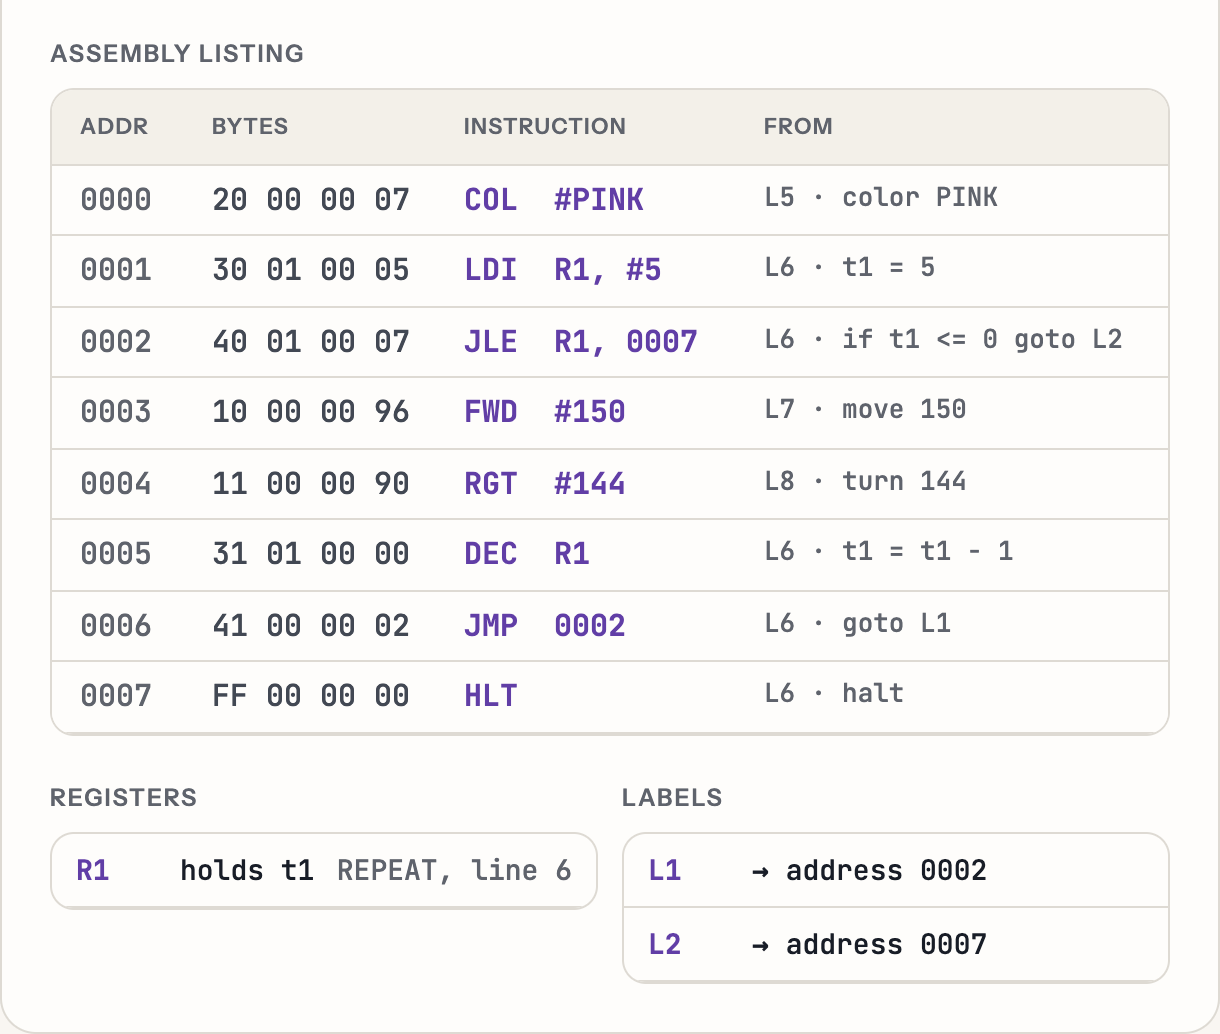
\includegraphics[width=\columnwidth]{figures/codegen-listing.png}
\caption{Machine code for the Star. Each row gives the address, the four bytes, the readable instruction and the three address instruction it came from. Below: the register holding the loop counter and the addresses of the two labels after backpatching.}
\label{fig:listing}
\end{figure}

The VM fetches the instruction at the program counter, executes it, and moves to the next address or to a jump target. \code{FWD} computes the new position from the heading with sine and cosine and records a line segment when the pen is down. A run stops at \code{HLT} or after two million steps, a guard that keeps any program from freezing the page. The Star runs in 29 steps: two setup instructions, five rounds of five instructions, the final test and the halt. The website can run the program one instruction at a time and shows the registers and the turtle state after each step (Fig.~\ref{fig:vm}).

\begin{figure*}[t]
\centering
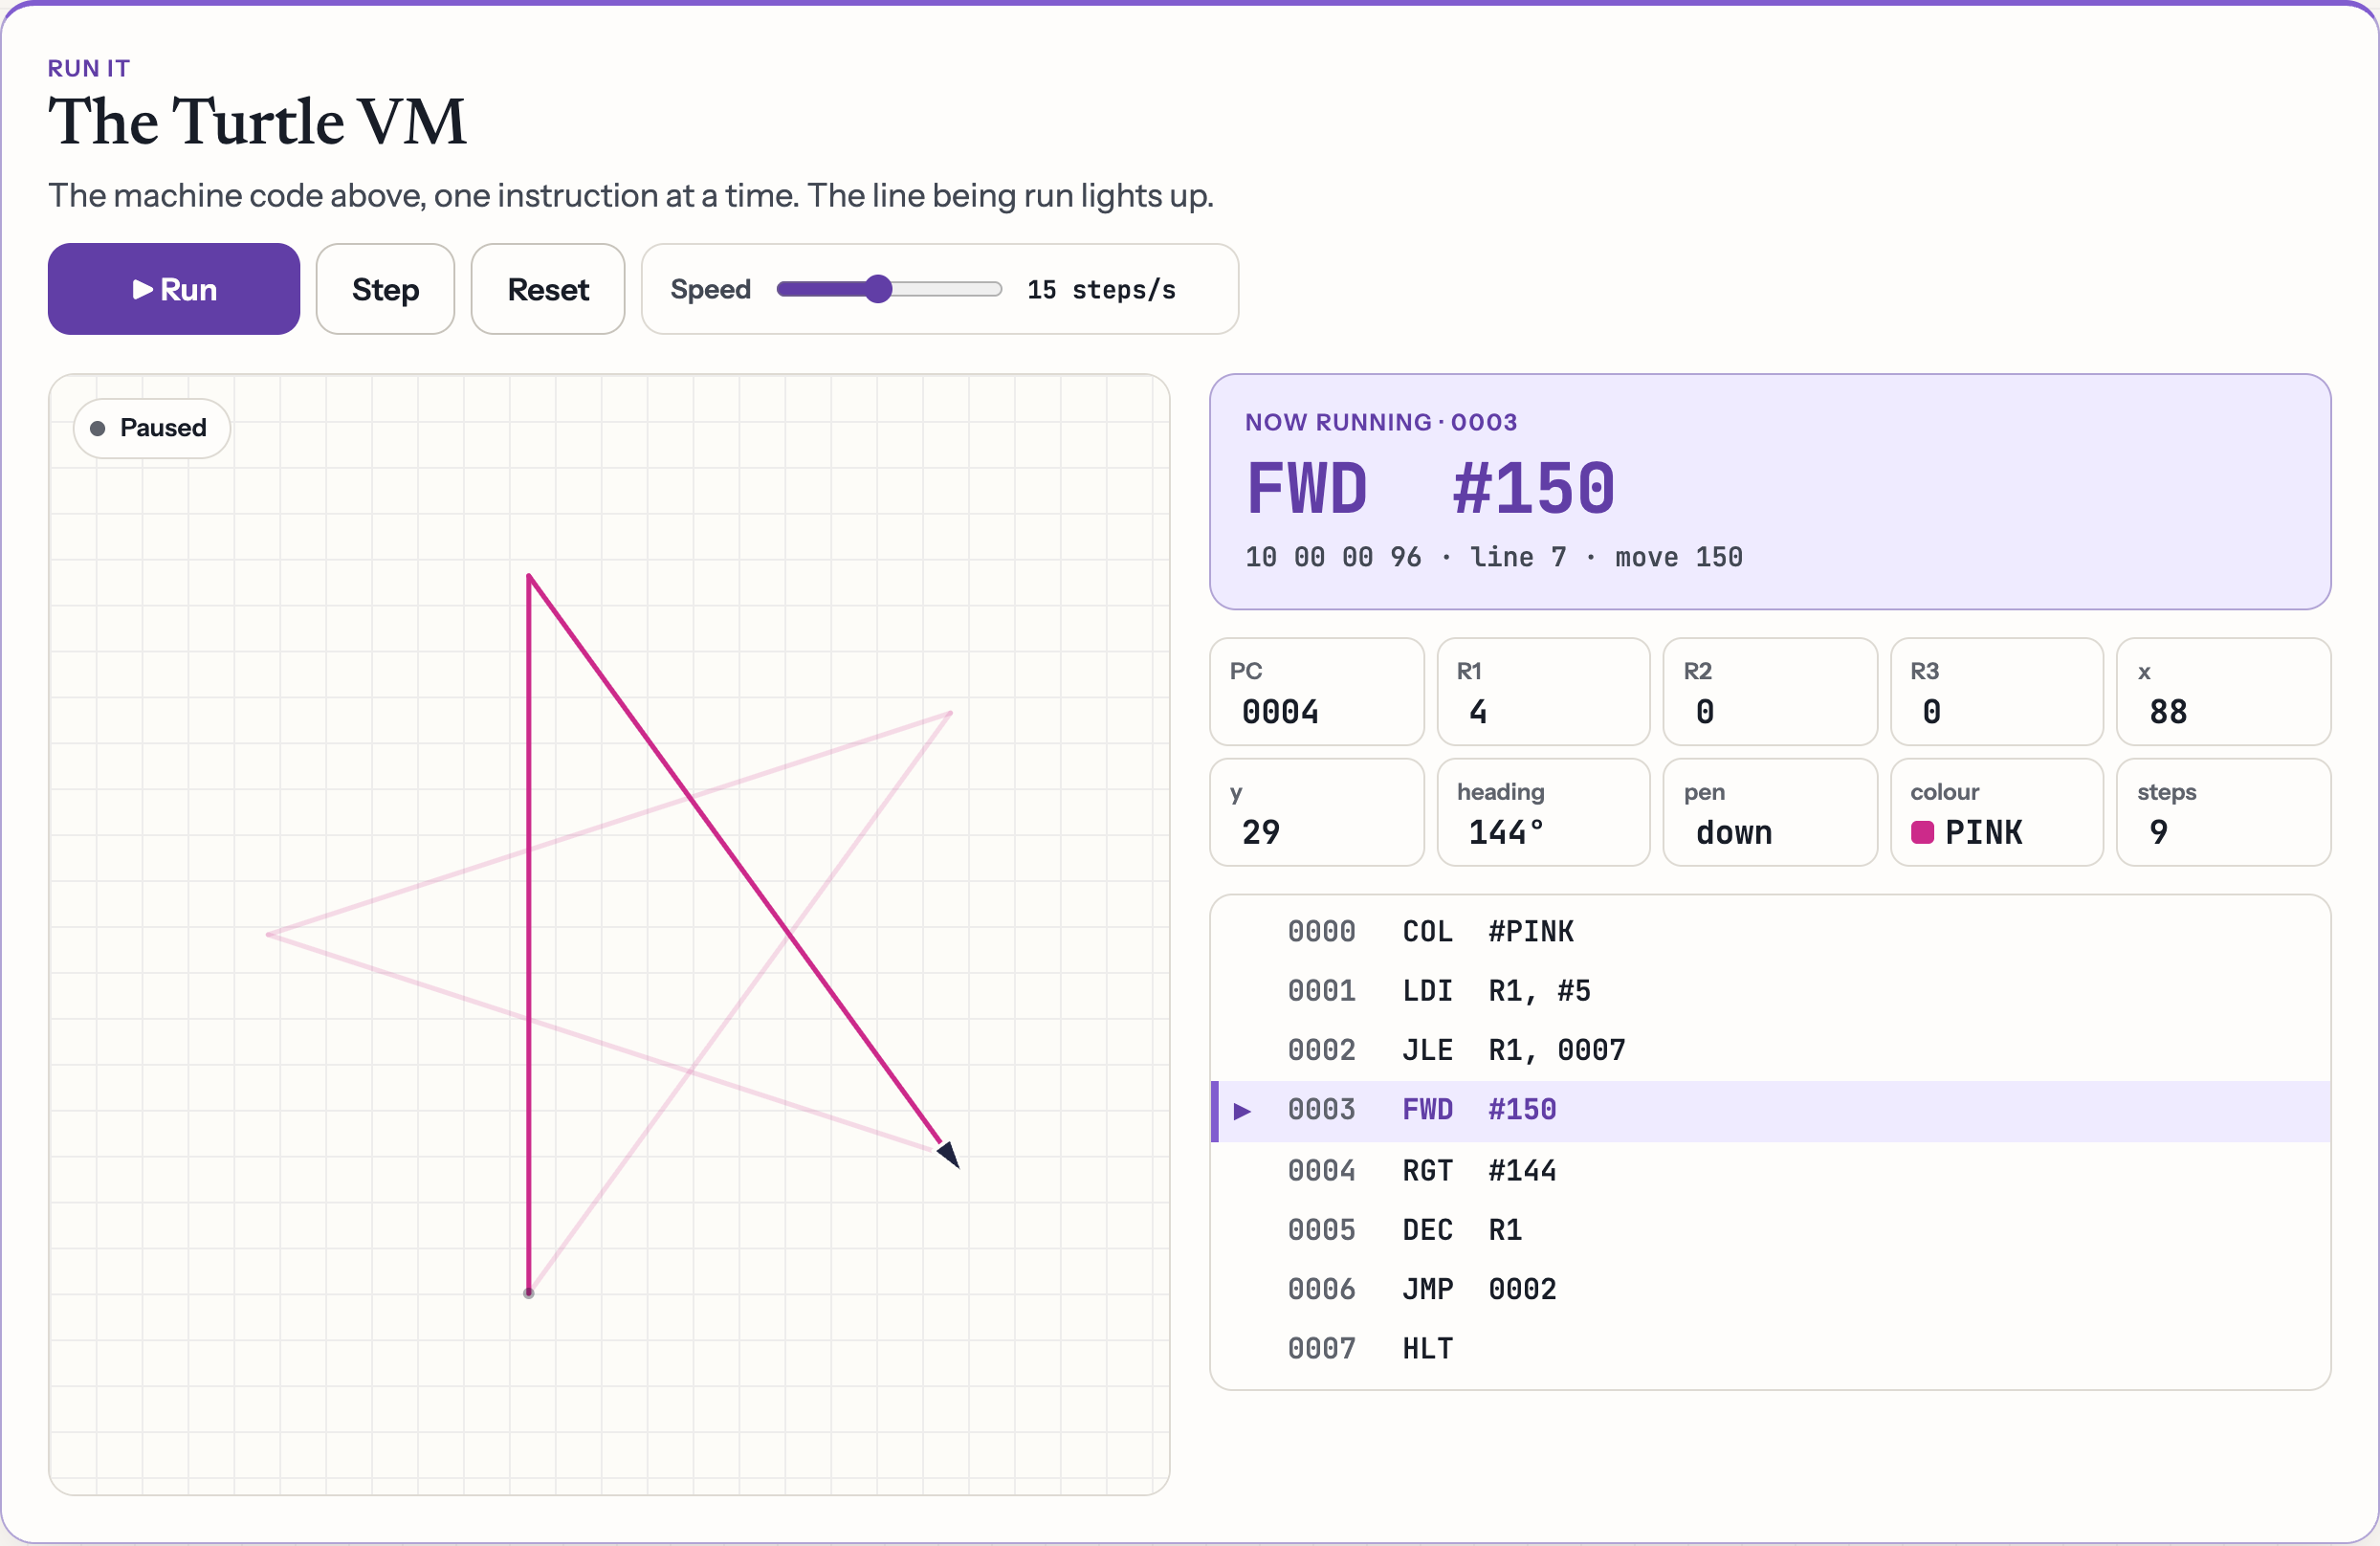
\includegraphics[width=0.86\textwidth]{figures/vm.png}
\caption{The Turtle VM paused after nine steps of the Star. The current instruction, \texttt{FWD \#150} at address 0003, is highlighted with its bytes and source line; R1 holds the remaining loop count. Lines already drawn are in full colour; the faint lines show the rest of the drawing.}
\label{fig:vm}
\end{figure*}

\section{Implementation}

The compiler module has 659 lines of plain JavaScript and no dependencies. It exports every phase, every rule table and the virtual machine, both as a CommonJS module and as a browser global. The website is built with Next.js and React and exported as static files, served from Cloudflare Pages; it sends nothing to a server, as the page itself is the compiler. Its interface was designed first as a set of design files and converted to React components by a small converter that we wrote.

The command line compiler, \code{turtlec}, has 444 lines. It prints a compact report of all six phases or any single phase in full, writes the drawing as SVG and the machine code as a binary file, and can load and run such a file after checking every opcode, register, colour and jump target. Errors name the file, line and column in the familiar form of command line compilers, with the source line, a caret under the error and a hint:

\begin{lstlisting}[style=plain]
examples/synerr.turtle:4:3: syntax error:
  Expected ; after "100" but found "TURN".
    4 |   TURN 90;
      |   ^~~~
      = hint: Every command ends with a semicolon.
\end{lstlisting}

A suite of ten tests, run with the Node.js test runner, covers every phase, the error programs, warnings, SVG output, and a round trip of machine code through a file.

\section{Evaluation}

We compiled the seven example programs in the repository: four valid programs and three that each fail in a different phase. Table~\ref{tab:eval} reports the valid programs. Times are the mean of 2000 complete compilations on an Apple M4 Pro with Node.js 25.6.1; each compilation includes both virtual machine runs used for the equivalence check.

\begin{table}[t]
\caption{Results on the four valid example programs. Tokens include the end marker; instructions are three address instructions without labels; steps are virtual machine steps.}
\label{tab:eval}
\centering
\footnotesize
\setlength{\tabcolsep}{3.2pt}
\resizebox{\columnwidth}{!}{%
\begin{tabular}{@{}l r r r r r r r@{}}
\toprule
\textbf{Program} & \textbf{Tokens} & \textbf{Parse} & \textbf{Checks} & \textbf{Instr.} & \textbf{Steps} & \textbf{Lines} & \textbf{Time} \\
 & & \textbf{steps} & & \textbf{before/after} & \textbf{before/after} & & \textbf{($\mu$s)} \\
\midrule
Square & 14 & 28 & 5 & 8 / 8 & 24 / 24 & 4 & 11.7 \\
Star & 25 & 46 & 9 & 11 / 8 & 35 / 29 & 5 & 20.7 \\
Flower & 26 & 49 & 10 & 14 / 13 & 316 / 316 & 48 & 42.4 \\
Playground & 47 & 89 & 20 & 24 / 10 & 67 / 36 & 7 & 49.8 \\
\bottomrule
\end{tabular}}
\end{table}

\emph{Optimization.} The optimizer reduced the Star from 11 to 8 instructions (27\%) and its run from 35 to 29 steps (17\%). On the playground, a program written so that every rule applies, all six rules fired and the code shrank from 24 to 10 instructions (58\%) and from 67 to 36 steps (46\%). On the Flower, O1 and O2 removed a constant copy; because copies emit no machine code, the step count did not change. The Square offered nothing to remove. In all four programs the equivalence check confirmed identical drawings.

\emph{Speed.} A complete compilation, all six phases plus two runs of the virtual machine, took between 11.7 and 49.8 microseconds. A display refreshes every 16 milliseconds at 60 frames per second, so recompiling on every keystroke costs well under one percent of a frame.

\emph{Error handling.} Each error program stopped in its intended phase with every error reported. The lexical demonstration produced 2 errors (an unknown character, and a detached minus sign) in 2.6 microseconds; the syntax demonstration produced 1 error, a missing semicolon, in 6.7 microseconds; and the semantic demonstration produced 4 errors under rules S3, S6, S4 and S1 in 8.2 microseconds.

\section{Limitations and Future Work}

The language is deliberately small. It has no arithmetic expressions, no variables that change, and no procedures, so many classic optimizations have nothing to act on. The parser stops at the first syntax error; panic mode recovery, skipping to the next semicolon, would let one run report several. The optimizer is local to straight line code and simple loops; loop unrolling and a drawn control flow graph are natural next steps. Three registers limit nesting to three levels; register spilling would remove that limit. Finally, an LR parser for the same grammar, shown beside the LL(1) parser, would let students compare the two families on one example.

\section{Conclusion}

Turtle Compiler shows one program passing through all six phases of a compiler, from characters to machine code to a picture, with the rules of each phase stated and their output visible. Keeping the language small made it possible to implement every phase completely in 659 lines and to present each phase in full on one screen. Checking every optimization against the unoptimized program on the virtual machine turned the claim that the optimizer preserves meaning into something the user can see on every compilation.

\section*{Acknowledgment}

This work was carried out as the course project for Compiler Design and Automata at Newton School of Technology, Rishihood University.

\begin{thebibliography}{10}

\bibitem{aho2006}
A.~V. Aho, M.~S. Lam, R.~Sethi, and J.~D. Ullman, \emph{Compilers: Principles, Techniques, and Tools}, 2nd~ed. Boston, MA, USA: Pearson Education, 2006.

\bibitem{cooper2011}
K.~D. Cooper and L.~Torczon, \emph{Engineering a Compiler}, 2nd~ed. Burlington, MA, USA: Morgan Kaufmann, 2011.

\bibitem{muchnick1997}
S.~S. Muchnick, \emph{Advanced Compiler Design and Implementation}. San Francisco, CA, USA: Morgan Kaufmann, 1997.

\bibitem{papert1980}
S.~Papert, \emph{Mindstorms: Children, Computers, and Powerful Ideas}. New York, NY, USA: Basic Books, 1980.

\bibitem{abelson1981}
H.~Abelson and A.~diSessa, \emph{Turtle Geometry: The Computer as a Medium for Exploring Mathematics}. Cambridge, MA, USA: MIT Press, 1981.

\bibitem{knuth1965}
D.~E. Knuth, ``On the translation of languages from left to right,'' \emph{Information and Control}, vol.~8, no.~6, pp.~607 to 639, 1965.

\bibitem{mckeeman1965}
W.~M. McKeeman, ``Peephole optimization,'' \emph{Communications of the ACM}, vol.~8, no.~7, pp.~443 to 444, 1965.

\bibitem{allen1970}
F.~E. Allen, ``Control flow analysis,'' \emph{ACM SIGPLAN Notices}, vol.~5, no.~7, pp.~1 to 19, 1970.

\bibitem{rodger2006}
S.~H. Rodger and T.~W. Finley, \emph{JFLAP: An Interactive Formal Languages and Automata Package}. Sudbury, MA, USA: Jones and Bartlett, 2006.

\end{thebibliography}

\end{document}
